\subsection{Electronics}

Before assembling the electronics on the wooden structure, we first created a \textbf{fully functional bench test setup} to validate our components and connections. This early prototype allowed us to test the behavior of the \textbf{DC motors with omnidirectional wheels} and the \textbf{ultrasonic sensors} in a controlled environment.

We mounted the three motors on metal brackets and connected them to their respective \textbf{DRV8871 motor drivers}. These, in turn, were wired to a breadboard where we centralized all the connections, including the \textbf{ATmega328P microcontroller}, \textbf{six HC-SR04 ultrasonic sensors}, and \textbf{power regulation circuits}. We used a laboratory power supply to ensure voltage stability during the tests.

\begin{figure}[H]
    \centering
    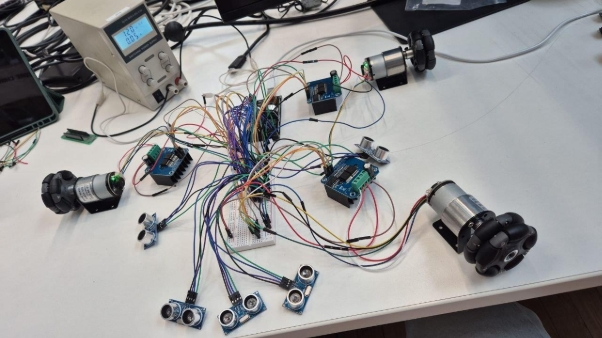
\includegraphics[width=0.6\linewidth]{../ReportMovementModule/images/Aspose.Words.728084da-df58-4b9d-a372-f65cffbdb23d.010.jpeg}
    \caption{Electronics Bench Test Setup}
\end{figure}

Once the behavior of the components was confirmed, we moved on to physically \textbf{assembling the electronics onto the wooden chassis}. The three motors were mounted onto the underside of the lower wooden base. Their positioning followed the triangular configuration defined in our design, ensuring balanced and effective omnidirectional movement.

Once the motors were secured, we constructed \textbf{custom wooden supports} on the upper side of the base to hold the \textbf{motor drivers} (DRV8871). These supports allowed us to fix the drivers in place, providing both accessibility and protection for the connections. With the mechanical and structural elements ready, we proceeded to \textbf{wire the motors to the drivers}, carefully routing the motor cables through openings in the base. This ensured that the wiring remained organized and out of the way of moving parts.

\begin{figure}[H]
    \centering
    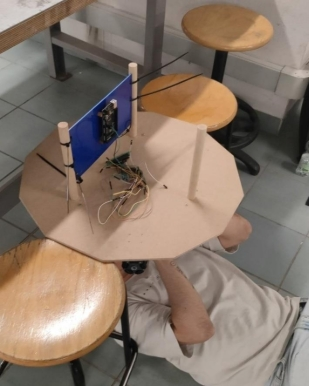
\includegraphics[width=0.6\linewidth]{../ReportMovementModule/images/Aspose.Words.728084da-df58-4b9d-a372-f65cffbdb23d.011.jpeg}
    \caption{Motor and Driver Setup}
\end{figure}

\begin{figure}[H]
    \centering
    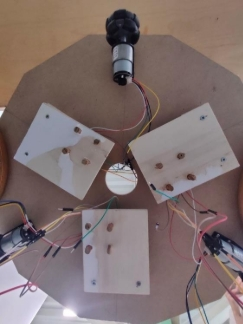
\includegraphics[width=0.6\linewidth]{../ReportMovementModule/images/Aspose.Words.728084da-df58-4b9d-a372-f65cffbdb23d.012.jpeg}
    \caption{Motor Driver Installation}
\end{figure}

The cables were then guided to the top layer of the chassis, where we placed the \textbf{microcontroller, power distribution components}, and \textbf{sensor modules}. The next step was to connect the \textbf{motor drivers to the microcontroller}, completing the control path between the motors and the logic unit. To organize this section of the circuit, we mounted the microcontroller onto a \textbf{vertical blue plastic panel} attached to the structure using zip ties. This panel allowed us to keep the wiring centralized, accessible, and separated from the moving parts below.

Once the core control system was in place, we installed the \textbf{ultrasonic sensors} around the robot perimeter. These were mounted on \textbf{alternating faces of the dodecagonal wooden base}, using custom white brackets to maintain stable orientation and optimal detection angles. The sensors were positioned to provide wide environmental coverage and were each connected to the microcontroller via dedicated digital pins.

\begin{figure}[H]
    \centering
    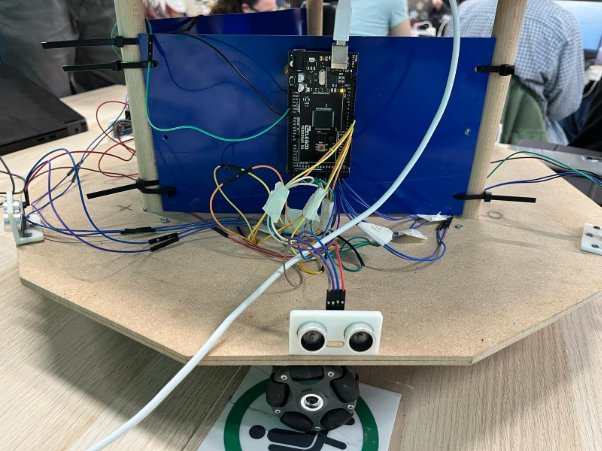
\includegraphics[width=0.6\linewidth]{../ReportMovementModule/images/Aspose.Words.728084da-df58-4b9d-a372-f65cffbdb23d.013.jpeg}
    \caption{Ultrasonic Sensor Installation}
\end{figure}

To manage power and grounding efficiently, we used \textbf{two small green protoboards} mounted on another blue panel. The \textbf{right-hand board} was used to \textbf{distribute power (VCC)} to all critical components, including the ultrasonic sensors, motor drivers, and microcontroller. The \textbf{left-hand board} was dedicated to \textbf{ground (GND) connections}, ensuring a common reference for the entire circuit. This setup allowed us to organize the wiring more cleanly, reduce loose connections, and centralize the power layout in a way that is both stable and maintainable.

\begin{figure}[H]
    \centering
    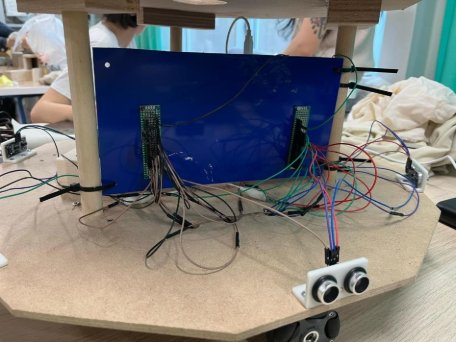
\includegraphics[width=0.6\linewidth]{../ReportMovementModule/images/Aspose.Words.728084da-df58-4b9d-a372-f65cffbdb23d.014.jpeg}
    \caption{Power Distribution Boards}
\end{figure}

To verify that the electronics were functioning correctly after assembly, we first powered the system using a \textbf{laboratory power supply}. This allowed us to set a precise voltage and current limit, ensuring a safe environment for initial testing and protecting the components from potential surges or wiring errors.

Once the wiring was confirmed and all components—motors, drivers, sensors, and microcontroller—responded as expected, we replaced the power supply with the robot's actual \textbf{LiFePO4 battery}. With the battery installed and secured to the base, we repeated the tests to confirm that the entire system could run autonomously on its intended power source. This step-by-step approach helped us detect and correct small connection issues early and ensured a smooth transition to portable, untethered operation.

\begin{figure}[H]
    \centering
    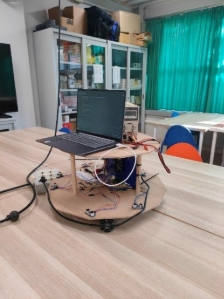
\includegraphics[width=0.6\linewidth]{../ReportMovementModule/images/Aspose.Words.728084da-df58-4b9d-a372-f65cffbdb23d.015.jpeg}
    \caption{Battery Installation}
\end{figure}

\begin{figure}[H]
    \centering
    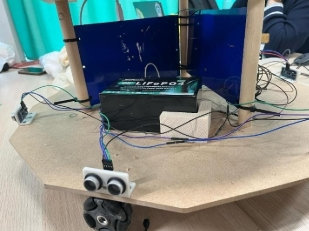
\includegraphics[width=0.6\linewidth]{../ReportMovementModule/images/Aspose.Words.728084da-df58-4b9d-a372-f65cffbdb23d.016.jpeg}
    \caption{Complete Electronics Assembly}
\end{figure}

Additionally, during the development process, we decided to incorporate a \textbf{camera module} into the system in order to enable docking with the charging station using \textbf{QR code detection}. This addition allowed the robot to recognize visual markers and orient itself toward the charging point when needed. Since this feature was not planned from the beginning, it was not included in the initial design phase. The decision to implement it emerged organically as the project evolved and we identified the need for more reliable and autonomous behavior during low-battery scenarios.

\begin{figure}[H]
    \centering
    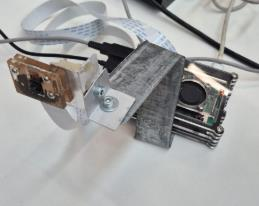
\includegraphics[width=0.6\linewidth]{../ReportMovementModule/images/Aspose.Words.728084da-df58-4b9d-a372-f65cffbdb23d.017.png}
    \caption{Camera Module Integration}
\end{figure}
